\section{Fundamentos de los sistemas difusos.}

\subsection{Introducción}
En los últimos años se han consolidado y aumentado las aplicaciones de la lógica difusa, abarcando sectores tan diversos como puede ser el control industrial, las búsquedas en bases de datos o estrategias de mantenimiento entre otros.

Como explican Carlos González [1] y Oscar G. et al. [2], las principales razones para tal proliferación de aplicaciones quizás sean la
sencillez conceptual de los Sistemas basados en Lógica Difusa, su facilidad
para adaptarse a casos particulares con pocas variaciones de parámetros,
su habilidad para combinar en forma unificada expresiones lingüísticas con
datos numéricos, el no requerir de algoritmos muy sofisticados para su
implementación o la automatización de tareas utilizando conocimiento experto.

La lógica tradicional (así como la teoría de conjuntos y el álgebra booleana) son isomorfas\footnote{\url{http://matematica.laguia2000.com/general/isomorfismo}}, bajo transformaciones adecuadas, es decir, tienen una estructura similar, lo cual significa que las definiciones hechas para cualquiera de las tres teorías se pueden llevar a las otras dos a través de transformaciones sencillas, mediante la correspondencia de operadores que se muestra en la \tableref{table:1}.



\begin{table}[h]
	\centering
	\begin{tabular}{@{}ccc@{}}
		\toprule
		\multicolumn{1}{l}{\textbf{Teoría de conjuntos}} & \multicolumn{1}{l}{\textbf{Álgebra booleana}} & \multicolumn{1}{l}{\textbf{Lógica tradicional}} \\ \midrule
		\multicolumn{1}{c}{Intersección}               & \multicolumn{1}{c}{Conjunción}               & \multicolumn{1}{c}{AND}                        \\ \midrule
		\multicolumn{1}{c}{Unión}                      & \multicolumn{1}{c}{Disyunción}               & \multicolumn{1}{c}{OR}                         \\ \midrule
		Complemento                                      & Negación                                      & NOT                                             \\ \bottomrule
	\end{tabular}
	\caption{Correspondencia entre operadores de la Teoría de Conjuntos, el Álgebra Booleana y la Lógica Tradicional.}
	\label{table:1}
\end{table}

\subsection{Teoría de conjuntos difusos}
Antes de comenzar con la definición de Conjuntos Difusos, veamos cómo se definen los conjuntos convencionales (Conjuntos Concretos).

Un conjunto concreto se define como una colección de elementos que
existen dentro de un Universo. Así, dado el universo U que consta de los números enteros no negativos menores que 10:

\texttt{U = \{0,1,2,3,4,5,6,7,8,9\}}

podemos definir algunos conjuntos como\\
\newline
\null\hspace{0.59cm}\texttt{A = \{0,2,4,6,8\}},\newline
\null\hspace{0.37cm}\texttt{B = \{1,3,5,7,9\}},\newline
\null\hspace{0.37cm}\texttt{C = \{1,4,7\}} \ldots

De esta forma, hemos establecido a qué conjuntos pertenecen cada uno de los elementos del universo \texttt{U}. Cada uno de estos conjuntos queda perfectamente definido si utilizamos una función de pertenencia (\texttt{u(x)}) sobre los elementos del universo \texttt{U} de forma que a cada elemento de \texttt{U} se le asigna un valor 1 o 0 en función de si pertenece o no a dicho conjunto.

Oscar G. et al. [2] nos plantean la siguiente función de pertenencia que define el conjunto \texttt{C}
\\ \newline
\null\hspace{0.59cm}\texttt{u\textsubscript{C}(0)} = 0;\\
\null\hspace{0.59cm}\texttt{u\textsubscript{C}(1)} = 1;\\
\null\hspace{0.59cm}\texttt{u\textsubscript{C}(2)} = 0;\\
\null\hspace{0.59cm}\texttt{u\textsubscript{C}(3)} = 0;\\
\null\hspace{0.59cm}\texttt{u\textsubscript{C}(4)} = 1;\\
\null\hspace{0.59cm}\texttt{u\textsubscript{C}(5)} = 0;\\
\null\hspace{0.59cm}\texttt{u\textsubscript{C}(6)} = 0;\\
\null\hspace{0.59cm}\texttt{u\textsubscript{C}(7)} = 1;\\
\null\hspace{0.59cm}\texttt{u\textsubscript{C}(8)} = 0;\\
\null\hspace{0.59cm}\texttt{u\textsubscript{C}(9)} = 0;

Un Conjunto difuso se define de forma similar, con una diferencia conceptual importante: un elemento puede pertenecer parcialmente a un conjunto. 

Continuemos con el universo \texttt{U} que definimos anteriormente.
Un conjunto difuso D definido sobre dicho universo podría ser el siguiente:
\\ \newline
\null\hspace{0.59cm}\texttt{C = \{0.2/1,0.5/4,1/7\}}

Con esta definición, estamos representando que el elemento 1 pertenece en un 20\% al
conjunto \texttt{C} (y por tanto pertenece en un 80\% al complemento de \texttt{C}), mientras que
que el elemento 4 pertenece en un 50\%, y el elemento 7 en un 100\% .

De igual forma que con los Conjuntos Concretos, podemos definir una función de pertenencia \texttt{u\textsubscript{C}(x)}:
\\ \newline
\null\hspace{0.59cm}\texttt{u\textsubscript{C}(0)} = 0.0;\\
\null\hspace{0.59cm}\texttt{u\textsubscript{C}(1)} = 0.2;\\
\null\hspace{0.59cm}\texttt{u\textsubscript{C}(2)} = 0.0;\\
\null\hspace{0.59cm}\texttt{u\textsubscript{C}(3)} = 0.0;\\
\null\hspace{0.59cm}\texttt{u\textsubscript{C}(4)} = 0.5;\\
\null\hspace{0.59cm}\texttt{u\textsubscript{C}(5)} = 0.0;\\
\null\hspace{0.59cm}\texttt{u\textsubscript{C}(6)} = 0.0;\\
\null\hspace{0.59cm}\texttt{u\textsubscript{C}(7)} = 1.0;\\
\null\hspace{0.59cm}\texttt{u\textsubscript{C}(8)} = 0.0;\\
\null\hspace{0.59cm}\texttt{u\textsubscript{C}(9)} = 0.0;

Como podemos ver, hay algunas diferencias sustanciales entre los Conjuntos Difusos y los Conjuntos Concretos:
\begin{itemize}
	\item La función de pertenencia asociada a los Conjuntos Concretos sólo puede
	tener dos valores: 1 ó 0, mientras que en los conjuntos difusos puede
	tener cualquier valor entre 0 y 1.
	\item Un elemento puede pertenecer (parcialmente) a un conjunto difuso y
	simultáneamente pertenecer (parcialmente) al complemento de dicho
	conjunto. Esto no es posible en los conjuntos concretos, ya que
	constituiría una violación al \textit{principio del tercero excluido.}\footnote{\url{https://es.wikipedia.org/wiki/Principio_del_tercero_excluido}}
	\item Las fronteras de un conjunto concreto son exactas, en tanto que las de
	un conjunto difuso son, precisamente, difusas, ya que existen elementos
	en las fronteras mismas, y estos elementos están a la vez dentro y fuera
	del conjunto.
\end{itemize}

No obstante, debemos tener en cuenta que:
\begin{itemize}
	\item Los Conjuntos Concretos son un caso particular de los Conjuntos Difusos.
	\item Cualquier conjunto es difuminable.
\end{itemize}

En el mundo real, el hecho de que un elemento pueda pertenecer parcialmente a un conjunto tiene numerosas ventajas, veamos un ejemplo:

\textit{Ejemplo 1:} Supóngase que se desea clasificar a los miembros de un equipo
de fútbol según su estatura en tres conjuntos, Bajos, Medianos y Altos.
Podría plantearse que se es Bajo si se tiene una estatura inferior a, por
ejemplo, 160 cm, que se es Mediano si la estatura es superior o igual a 160
cm e inferior a 180 cm, y se es alto si la estatura es superior o igual a 180
cm, con lo que se lograría una clasificación en conjuntos concretos. \label{ej:1}

Sin embargo, ¿es tan significativa la diferencia entre un jugador con estatura 179.9 cm y otro de 180 cm? ¿Ese milímetro representa una diferencia tan significativa que tenemos que clasificar a los jugadores en dos conjuntos distintos? Utilizando Conjuntos Concretos uno es alto y otro es mediano.

Si se optase por efectuar la misma
clasificación con conjuntos difusos estos cambios abruptos se evitarían,
debido a que las fronteras entre los conjuntos permitirían cambios graduales
en la clasificación.

\begin{figure}[H]
	\centering
	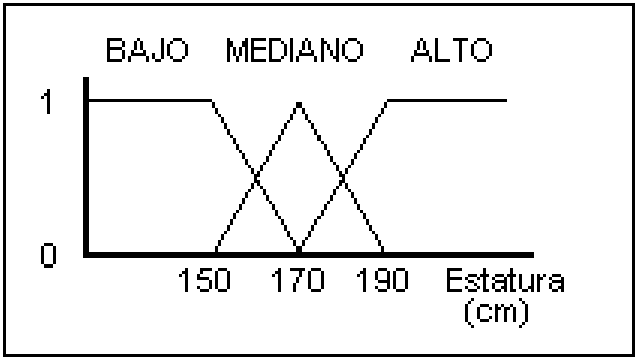
\includegraphics[scale=0.3]{images/fuzzy_example.png}
	\caption{Funciones de pertenencia del ejemplo 1}
	\label{fig:ej1}
\end{figure}
La \figureref{fig:ej1} muestra cómo podría hacerse dicha clasificación: el universo de
discurso sería el conjunto continuo de todas las posibles estaturas (el
intervalo [130,210]cm por ejemplo). 

\begin{figure}[H]
	\centering
	\begin{subfigure}[b]{0.4\textwidth}
		\centering
		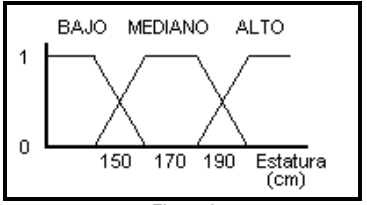
\includegraphics[scale = 0.5]{images/fuzzy_example_alt1.png}
		\caption{Representación alternativa del ejemplo 1}
		\label{fig:fuzzy1}
	\end{subfigure}
	~ %add desired spacing between images, e. g. ~, \quad, \qquad, \hfill etc. 
	%(or a blank line to force the subfigure onto a new line)
	\begin{subfigure}[b]{0.4\textwidth}
		\centering
		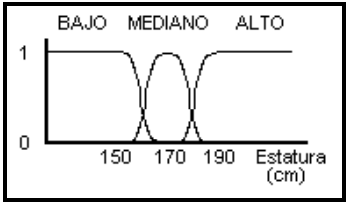
\includegraphics[scale = 0.5]{images/fuzzy_example_alt2.png}
		\caption{Representación alternativa del ejemplo 1}
		\label{fig:fuzzy2}
	\end{subfigure}
	\label{fig:alternativas}	
\end{figure}
La forma de
estas funciones de pertenencia no debe ser necesariamente la de la \figureref{fig:ej1},
pues depende de lo que se entienda por ``Bajo'', ``Mediano'' y ``Alto''.
En las \textit{figuras \ref{fig:fuzzy1} y \ref{fig:fuzzy2}} podemos ver otras alternativas para representar dichas funciones.

\subsection{Inferencia en lógica difusa}
La Inferencia lógica consiste en la combinación de proposiciones para
producir nuevas proposiciones. Así, al combinar la proposición \texttt{``X es A''} con
la proposición \texttt{``IF X es A THEN Y es B''}, se puede inferir la proposición \texttt{``Y es
B''} (ver \figureref{fig:inf}).

\begin{figure}[H]
	\centering
	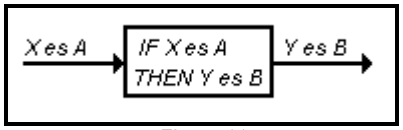
\includegraphics[scale=0.5]{images/logica_difusa.png}
	\caption{Inferencia en lógica tradicional.}
	\label{fig:inf}
\end{figure}

Una inferencia como ésta sólo es posible en
la lógica tradicional si la primera proposición \texttt{(``X es A'')} es idéntica a la
primera parte de la segunda proposición \texttt{(``(IF) X es A'')}; sin embargo, en la
lógica difusa estas dos proposiciones no deben ser necesariamente
idénticas, debido a que las fronteras de los conjuntos no son precisas. Así, al
combinar la proposición \texttt{``X es A*''} con la proposición \texttt{``IF X es A THEN Y es
B''}, puede obtenerse la proposición \texttt{``Y es B*''} (ver figura \figureref{fig:inf1}).

\begin{figure}[H]
	\centering
	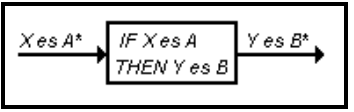
\includegraphics[scale=0.67]{images/logica_difusa_1.png}
	\caption{Inferencia en lógica difusa.}
	\label{fig:inf1}
\end{figure}

En la \figureref{fig:inferencia} podemos ver los mecanismos de Inferencia en Lógica Difusa \footnote{\url{http://www.cs.princeton.edu/courses/archive/fall07/cos436/HIDDEN/Knapp/fuzzy004.htm}}

\begin{figure}[H]
	\centering
	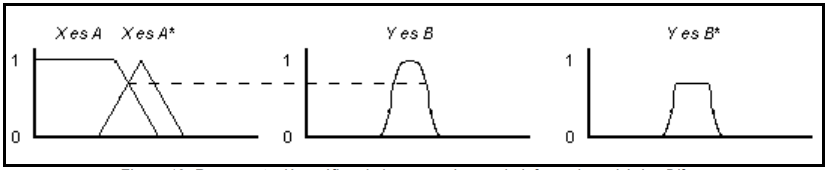
\includegraphics[scale=0.67]{images/mecanismos_inferencias_logica_difusa.png}
	\caption{Representación gráfica de los mecanismos de Inferencia en Lógica Difusa}
	\label{fig:inferencia}
\end{figure}

\subsection{Sistemas de lógica difusa}
Los mecanismos de Inferencia permiten simular el proceso de decisión humano utilizando implicaciones difusas y reglas de inferencia de lógica difusa. Un Sistema de Lógica Difusa aprovecha estos mecanismos como motor de cálculo de un sistema cuyas entradas y salidas son números concretos.

En la \figureref{fig:sistemas_difusos} podemos ver la estructura básica de un Sistema de Lógica difusa. El
sistema recibe varias entradas numéricas y entrega varias salidas numéricas. El bloque Difusor
se encarga de convertir las entradas numéricas no difusas en datos difusos, las cuales indican su grado de pertenencia a cada conjunto.
Estos datos son entregados al bloque Máquina de Inferencia que, utilizando las reglas de la forma \texttt{IF... THEN...} almacenadas en la Base de Reglas, produce una o más salidas difusas para que el bloque Concresor las convierta en salidas numéricas concretas.

\begin{figure}[H]
	\centering
	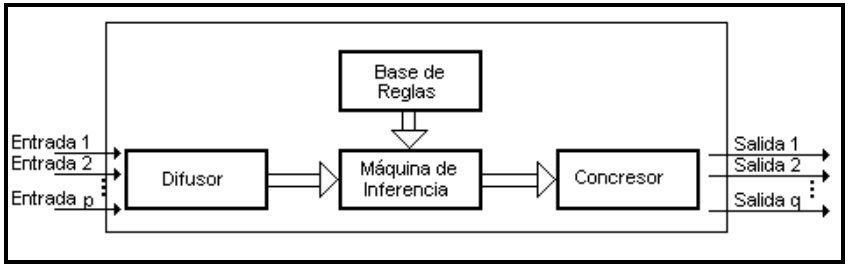
\includegraphics[scale=0.67]{images/sistemas_difusos.png}
	\caption{Estructura de un Sistema de Lógica Difusa}
	\label{fig:sistemas_difusos}
\end{figure}


Cada una de las variables de entrada y de salida tiene una representación
dentro del Sistema de Lógica Difusa en forma de Variables Lingüísticas. Una
variable lingüística tiene, entre otras cosas, una colección de valores que
puede adquirir la variable, y cada valor está representado por un conjunto
difuso. Así, retomando el ejemplo de la \figureref{fig:ej1}, la variable Estatura tendría
tres valores, Bajo, Mediano y Alto, y cada uno de estos valores estaría
representado por el conjunto difuso respectivo de la \figureref{fig:ej1}. Estos valores
reciben el nombre de Valores Lingüísticos.